\graphicspath{ {./figures/} }

\section{Background \& Research}
    \label{chap:background}
    \subsection{Small(Kat) Beginnings}
        The SmallKat project started in October 2017 as an Independent Study Project (ISP) with Worcester Polytechnic Institute (WPI) Professor Ciaraldi. The original intention of the project was to create the smallest possible walking quadruped we could in a single term. Using a digital 9 gram servo and a custom circuit board as the back bone of the project we were able to create a 16 degree of freedom system that very much resembled a feline. The first version barely walked and while ultimately the results of this project were quite successful, it left us wanting a much better solution. During the summer of 2018 we continued the project creating a slightly larger more advanced system. This version dubbed SmallKat V2 was significantly more successful than its predecsesor. It was more reliably designed and used much more reliable servo motors and several sensors including IMUs, pressure sensitive feet and current sensing. Additionally a reliable static walking gait was created and tested allowing it become WPI's most successful quadrupedal robotic system. Two versions of SmallKat V2 were built, aptly named Crimson and Gray they have been demoed at many of WPI's undergraduate robotics demonstrations. 
        
        \begin{figure}[H]
            \centering
            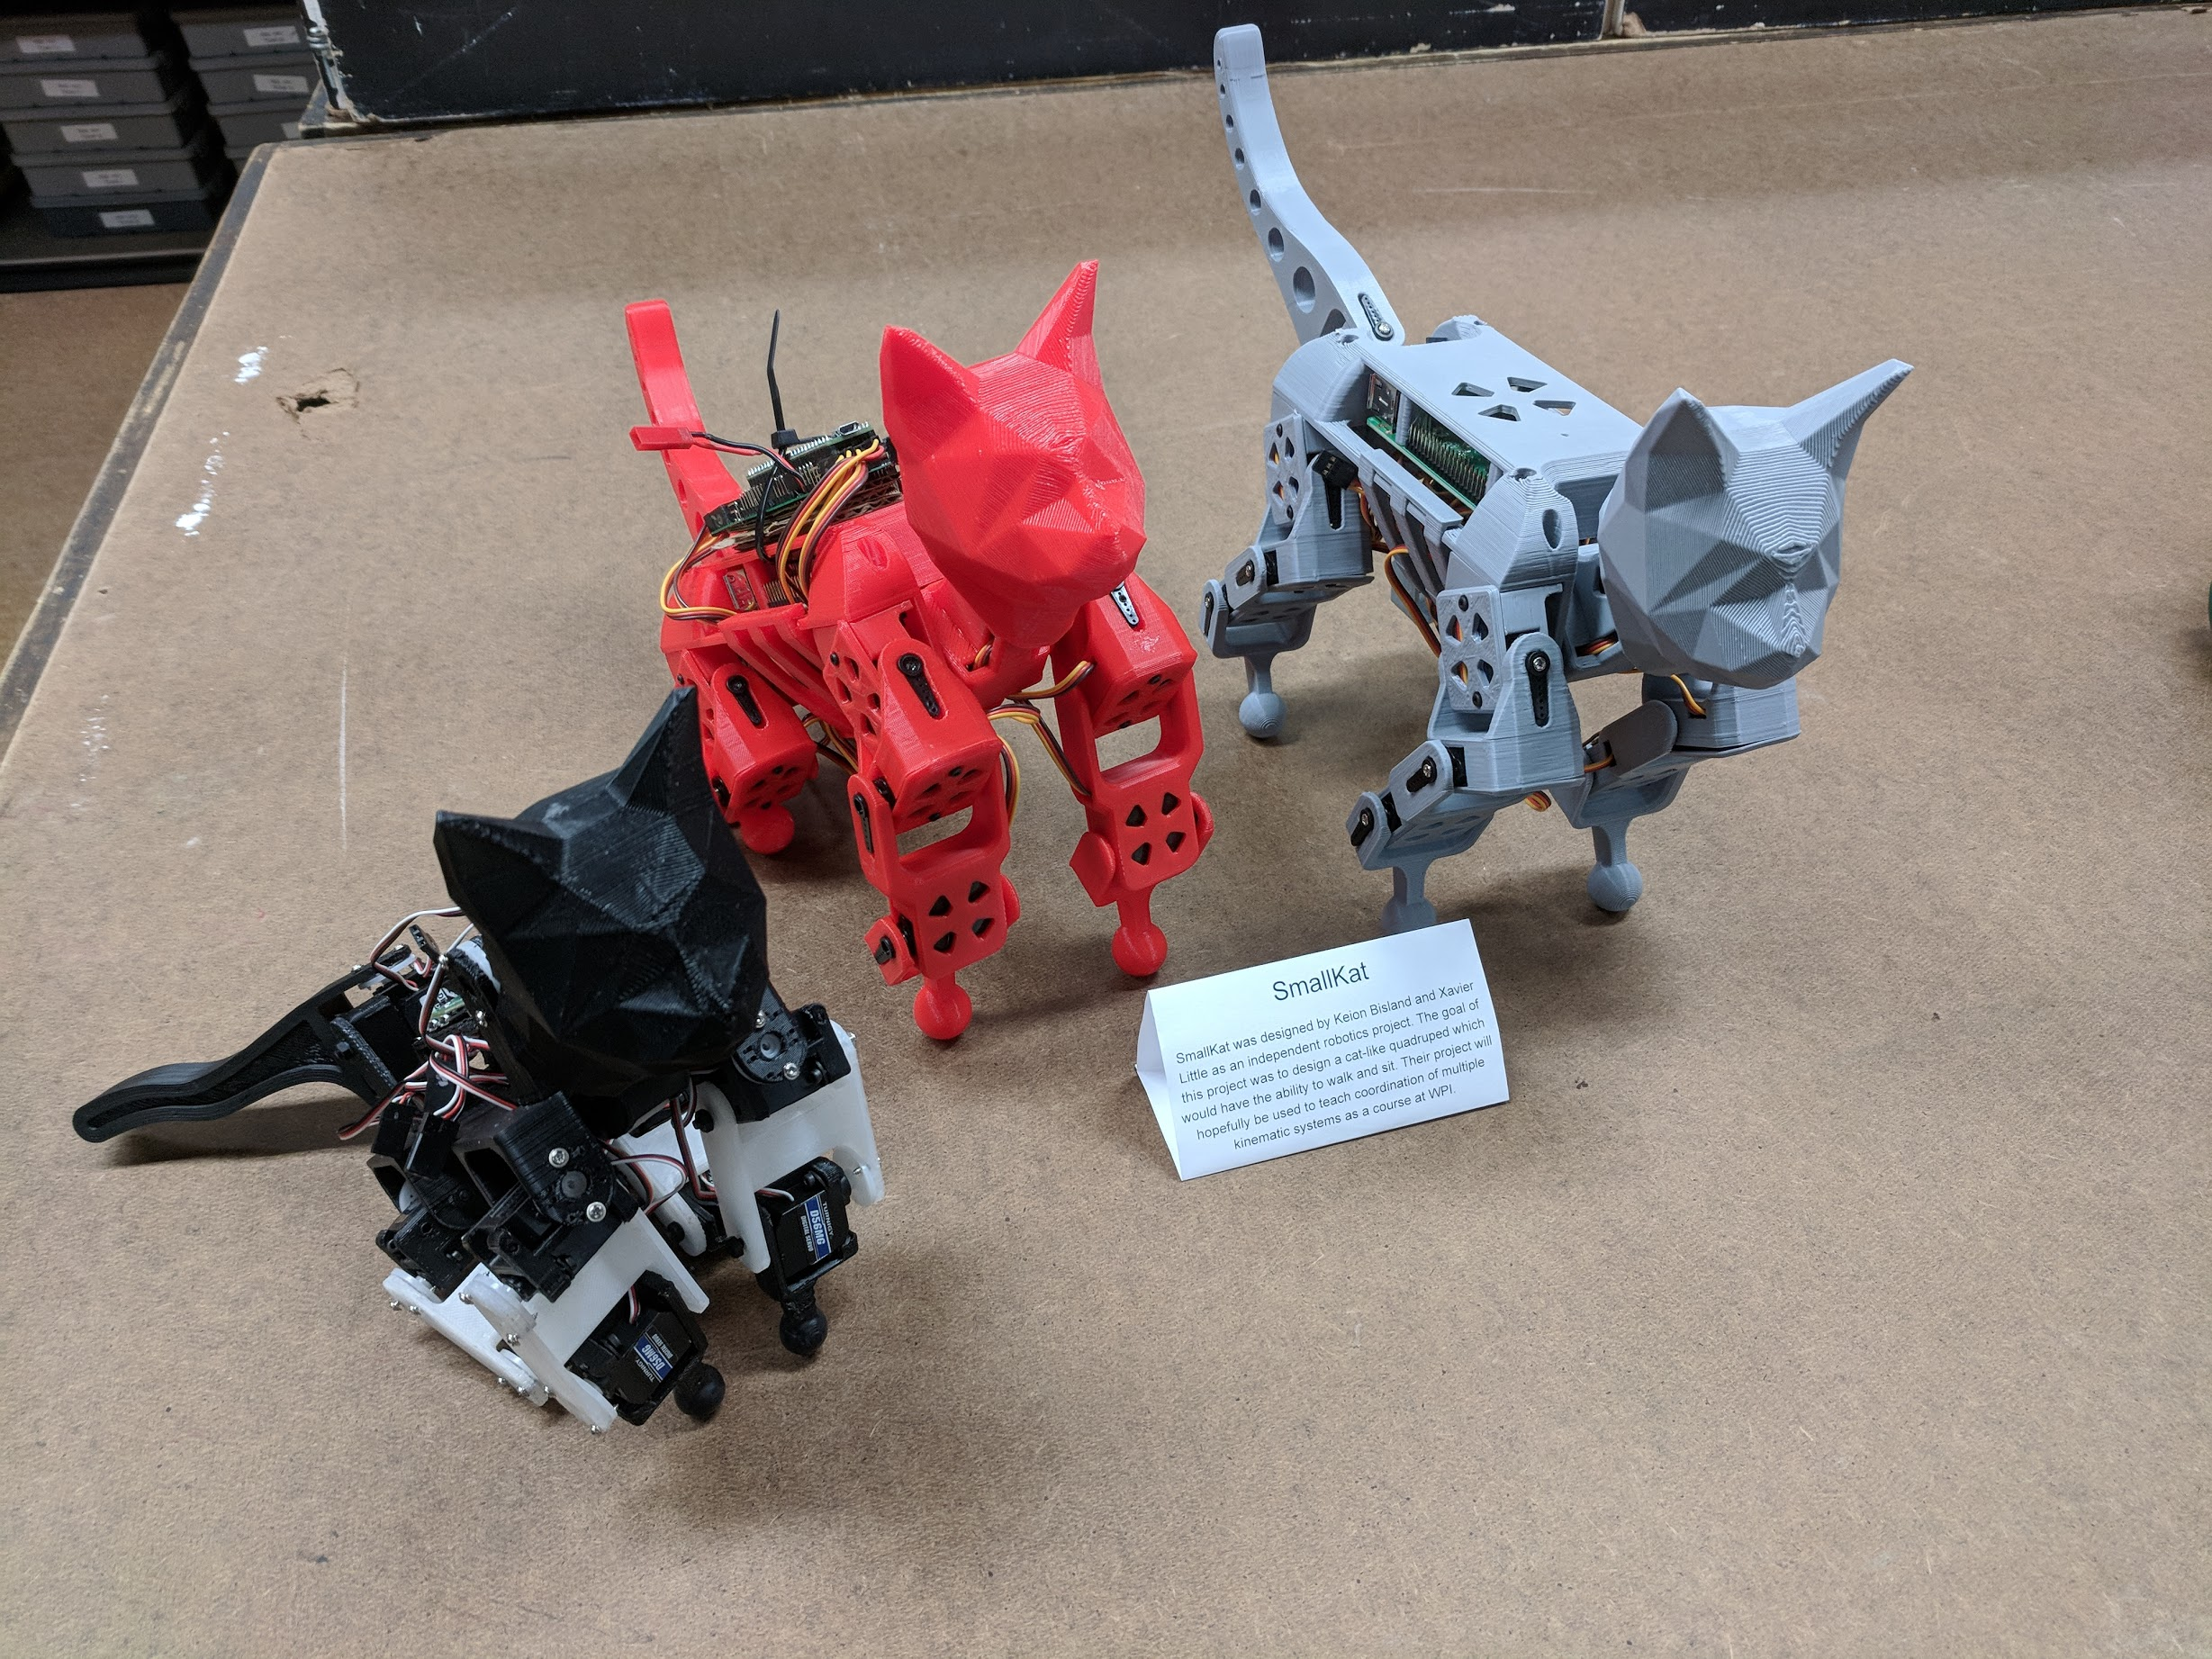
\includegraphics[width=120mm]{figures/V1andV2.jpg}
            \caption{SmallKat Versions 1, 2 and 2.1 during an undergraduate robotics lab demonstration}
            \label{fig:SmallKatVersions}
        \end{figure}
    \subsubsection{SmallKat V1 \& V2}
        \paragraph{Electrical}
        Developing V1 \& V2 of the SmallKat project revealed a lot of nuances when it came to the electrical system. These stemmed from the lack of any form of fed back due to the limited capabilities of using PWM and hobby servos. On V1 we had a very simplistic motherboard, just enough to get the system working. The purpose of the board was to breakout the 22 servo ports available on the Teensy 3.5 micro-controller as well as regulate the 7.4-8.4v input from the battery to 5v for the Teensy and the raspberry pi zero. This board made connecting all 16 Servos much easier and cleaner. When developing the motherboard for V2 a lot more time was taken to consider the possibilities of what could be achieved from the motherboard. On version 2, USB communication between the Raspberry Pi 3 B+ and the Teensy 3.5 was used to increase communication speed. IMUs were implemented at the front and rear of the robot along with current sensors for each of the 16 motor. Integration of these sensors were our attempt to combat the lack of feedback from our system. While we still had no direct positional or velocity feed back from the motors we could still attempt to implement a rough closed loop control using IMU data or determine the torque on the motors using the current sensing. Additional pressure sensors were added in the feet to detect when the robot was in contact with the ground. Due to time constraints these sensors have yet to be fully implemented into the control system of SmallKat V2.
        
        \paragraph{Software}
            \subparagraph*{Embedded}
            The Teensy 3.5 was programmed and developed through the Arduino environment. This was done in order to reduce the development time. However, this resulted in a number of issues arising. Because the target market for the Arduino environment is primarily beginners and hobbyists, there exist a great number of unnecessary checks and even more unnecessary layers of abstraction. This inadvertently limited the speed we could run the robot at. Many issues with using 16 PWM channels also arose at different points in the project as the platform is only designed to handle 12 by default, this meant a number of internal libraries had to be modified before the motors would move as expected. 
            \subparagraph*{Kinematics and Dynamics}
            For the higher level control of the robot a program called Bowler Studio was used. This program was developed by WPI graduate and Undergraduate Robotics Lab Manger Kevin Harrington. All the kinematic, dynamic and trajectory planning calculations were done using Bowler and then sent to the robots using the HID protocol over USB. Due to this program being in an early Beta stage there were a number of bugs that slowed the progress of the project. However having the developer of the program as an advisor to the project many of these were resolved quickly and/or could be be worked around relatively easily. This solution proved to be quite easy to use and allowed us to quickly develop a basic static walking gait. 
            % Need to cite Bowler Studio in this paragraph
        \paragraph{Mechanical Design}
        the mechanical aspect of the SmallKat system is centered around the servo for the system. For version 1 we used a small 9 gram digital servo. These provided a high amount of torque for their size. However they had a tendency to seize up if they were rotated not under their own power. Additionally the plastic used to house them was brittle and the small flanges used to hold them in place would often break. Other design flaws of the V1 system included hard to reach bolts and cheap screws used to connect each link to the servo horn. These screws would often strip when removed which happened often because the links would have to be adjusted. Version 2 fixed many of these problems. The servos were held inside each link with a cover instead of bolting through the flanges. Additionally a thin straight lever arm was used to connect each joint to the servo. This was pressed on after the link was already installed allowing for it to be easily adjusted. From version 1 to 2 the overall design and look didn't change. The robot had 4 legs wit 3 degrees of freedom and were situated underneath the body along with movable head and tail. While very similar in design to other quadrupedal systems The cat like features brought a smile to many faces.
        \subsubsection{SmallKat V3}
        The SmallKat MQP is the next evolution of the SmallKat quadruped series. Based on our prior work we are looking to create a new quadruped with more advanced systems than the previous two versions to allow  us to experiment with more complicated walking gaits and control systems.

    \subsection{Other Quadrupedal Robots}
    Boston Dynamics is currently one of the leaders in quadrupedal and bipedal systems. Their robots are the source of much inspiration for people attempting to create quadruped systems. They have created a variety of quadrupeds each with different capabilities. However, the quadruped research space has been expanding quickly, and new players have arrived to the scene.
    \paragraph{Boston Dynamics’ Spot Mini}
    SpotMini is a quadruped system designed and built by Boston Dynamics. It is a small agile system intended to be used in a variety of applications such as the home, office or outdoors. It stands at .83 meters tall and weighs 25kg. SpotMini is all-electric and can go for about 90 minutes on a single charge, depending on what it is doing.
    \begin{figure}[H]
        \centering
        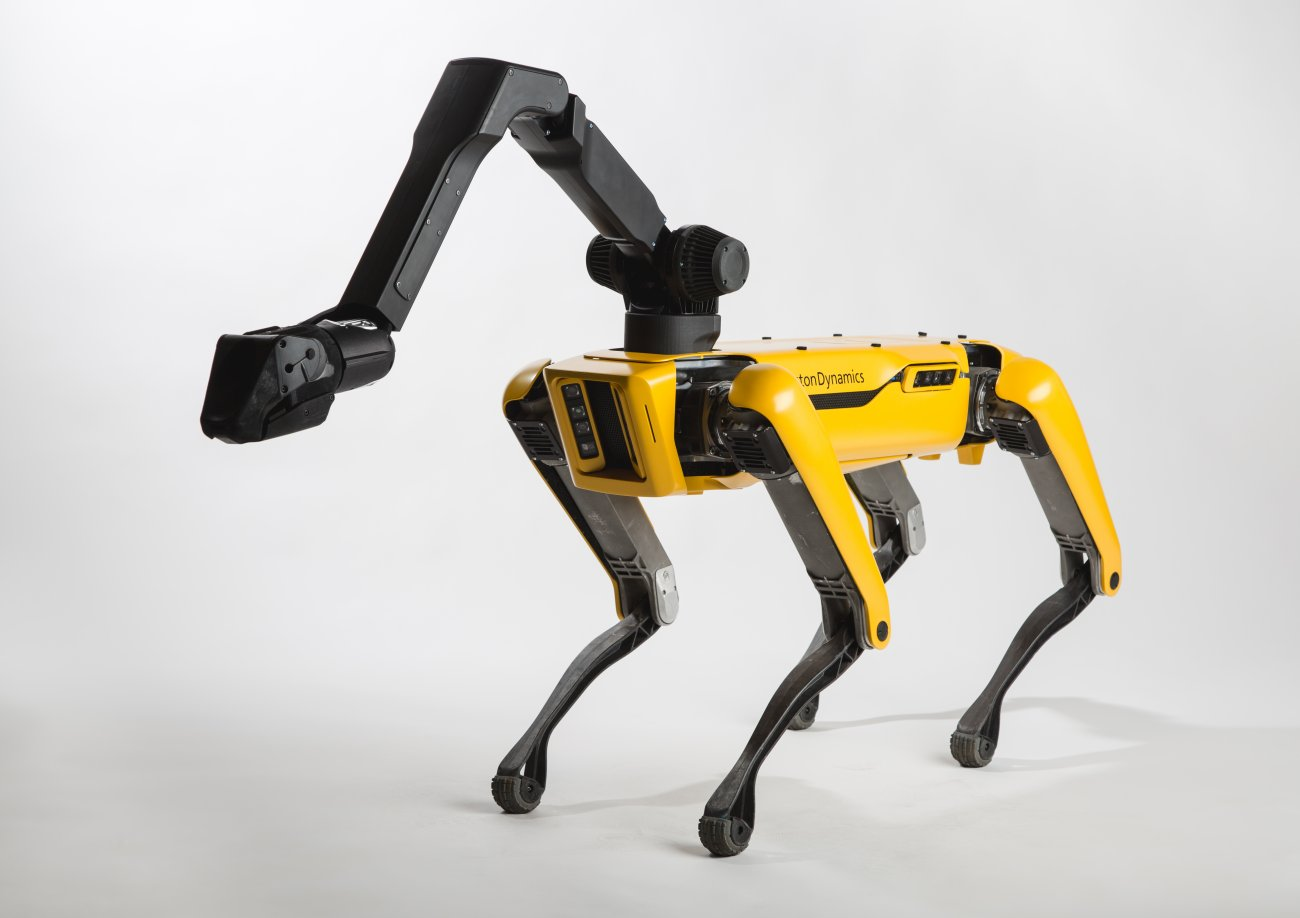
\includegraphics[width=0.7\linewidth]{figures/SpotMiniwithArm.jpg}
        \caption{Spot Mini with Arm}
        \label{fig:SpotMiniWithArm}
    \end{figure}
    SpotMini uses 4, 3 DOF legs to move itself around. It sports a 5kg, 5 DOF arm that it can use to pick things up and open doors. The sensor suite on board SpotMini and includes stereo cameras, depth cameras, an IMU, and position/force sensors in the limbs. These sensors help with navigation and mobile manipulation. SpotMini's dynamic control is unparalleled by any other quadruped system. The robot's movement is fluid and almost life like and it is able to navigate complex terrain and stairs. SpotMini can often be seen on YouTube were Boston Dynamics posts the robots new abilities and accomplishments. They plan on being able to commercial produce spot mini as a research platforms and for use in offices and homes.
    
    \paragraph{MITs Cheetah 3}
    One of the leaders of the quadruped world is Massachusetts Institute of Technology (MIT) Cheetah 3, the latest in MIT's Cheetah line. This quadrupedal walking system weighs just about 90lbs, and can run at a maximum of 13 feet per second. It has even demonstrated jumping onto platforms 30 inches tall and back-flipping!
    However, MIT Cheetah's most impressive feat is their dynamic controller. It can walk up stairs and rough terrain without the use of perception sensors, like 3D cameras and/or LIDARS. This technology was developed to help the robots maneuver successfully even when sensor data may not be perfect. MIT hopes that its Cheetah may one day provide disaster relief to areas where human access is difficult or dangerous. % Add sources
    \begin{figure}[H]
        \centering
        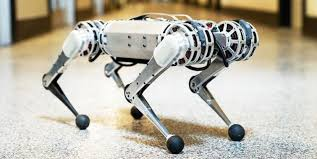
\includegraphics[width=0.7\linewidth]{figures/MITCheetah.jpeg}
        \caption{MIT's Cheetah 3}
        \label{fig:MITCheetah}
    \end{figure}

    \paragraph{Nybble} % https://www.indiegogo.com/projects/nybble-world-s-cutest-open-source-robotic-kitten#/
    Nybble by Petoi is a very new player in the world of quadrupeds, announced in late 2018 on Indegogo. It is designed to be a low-cost Arduino powered robot for hobbyists. It is entirely made out of laser-cut wood pieces and 9 gram servo motors, and is powered by a custom board with an ATmega328P chip (from an Arduino Uno). Each leg has 2 degrees of freedom, forming a planar manipulator. This prevents Nybble from being able to turn effectively or to walk dynamically, absorbing rough terrain or external forces. Along with a 1 DoF tail, Nybble is only really suitable for hobbyists and low end research.\cite{nybble}
    \begin{figure} [H]
        \centering
        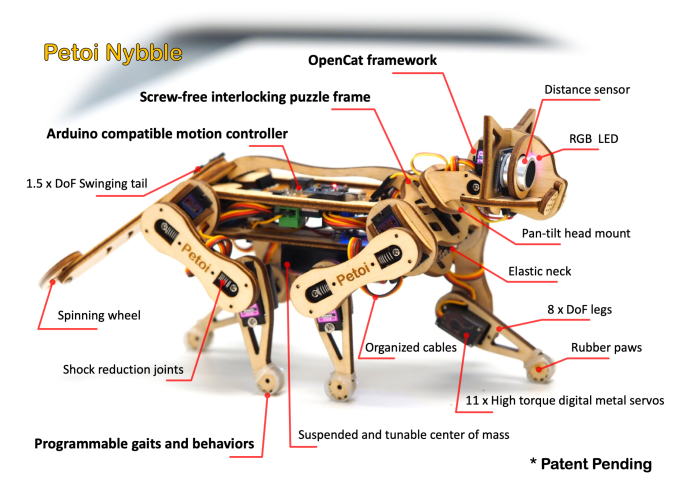
\includegraphics[width=0.7\linewidth]{figures/Nybble.png}
        \caption{Nybble's components}
    \end{figure}

    \subsection{Key Concepts} %% Maybe change the name?d
        \subsubsection{The Denavit-Hartenberg Convention}
            In mechanical engineering and robotics, DH parameters are the four parameters associated with a particular convention for attaching reference frames to the links of a spatial kinematic chain, or serial robot manipulator.
            \begin{figure}[H]
                \centering
                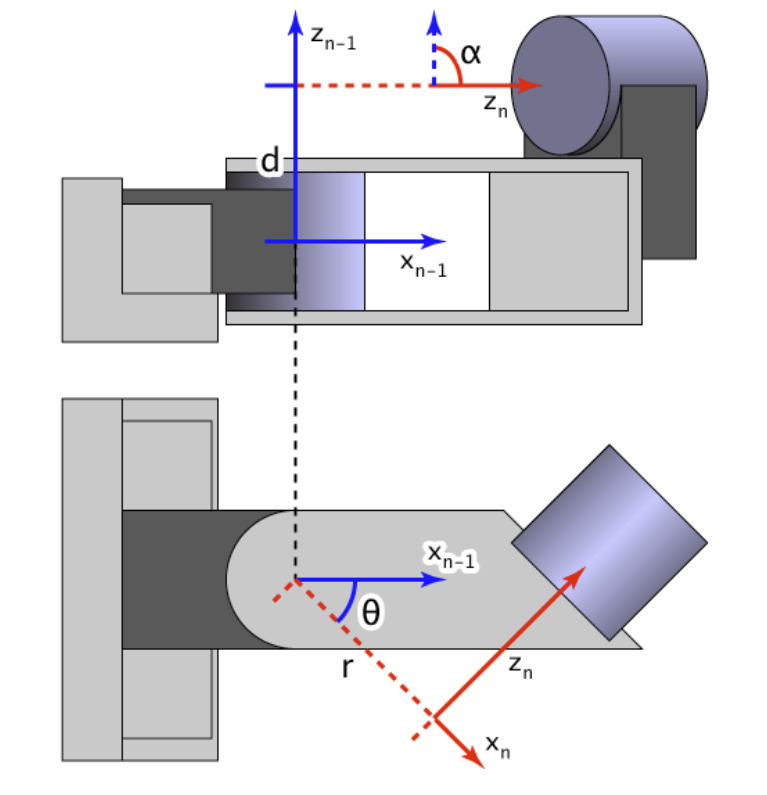
\includegraphics[width=75mm]{Dh.PNG}
                \caption{Visual Representation of DH parameters}
                \label{fig:DHParams_Visual}
            \end{figure}
            Coordinate frames are attached to the joints between two links such that one transformation is associated with the joint, [Z], and the second is associated with the link [X]. The coordinate transformations along a serial robot consisting of n links form the kinematics equations of the robot. At its core D-H parameters are coordinate frames attached to the joints between two links such that one transformation is associated with the joint denoted as Z, and the other is associated with the link denoted as X. By multiplying these together you can describe a single link and its joint in a robot manipulator. The coordinate transformations along an entire serial robot consisting of n links form the kinematics equations of the robot.
            \begin{equation}
            [T] = [Z_1][X_1][Z_2][X_2]...[X_{n-1}][Z_n][X_n]
            \end{equation}
            The coordinate transformations [Z] and [X], are determined by modeling the joints connecting the links as either hinged or sliding joints. By doing this, each of the joints can then be further described by a unique line S in space that forms the joint axis and define the relative movement of the two links. A typical serial robot is characterized by a sequence of these lines. For example in a six degree of freedom serial manipulator there are six Si where i = 1,...,6, one for each joint in the robot. For each sequence of lines Si and Si+1, there is a common normal line Ai,i+1. The system of six joint axes Si and five common normal lines Ai,i+1 form the kinematic skeleton of this six degree of freedom serial robot. Denavit and Hartenberg introduced the convention that Z coordinate axes are assigned to the joint axes Si and X coordinate axes are assigned to the common normals Ai,i+1.

            This convention allows the definition of the movement of links around a common joint axis Si by the screw displacement,
            \begin{figure}[H]
                \centering
                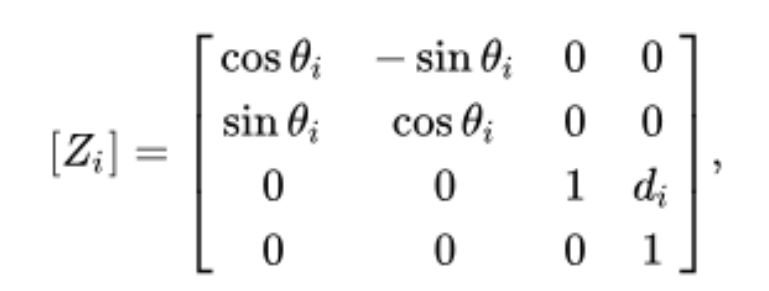
\includegraphics[width=0.7\textwidth]{zframe.PNG}
                \caption{Rotation Matrix for Z axis}t
                \label{fig:RotationMatrixZAxis}
            \end{figure}
            where $\theta$i is the rotation around and di is the slide along the Z axis. Depending on how the robot is constructed either of the parameters $\theta$ or d can be constants. The dimensions of each link in the serial chain are defined by the screw displacement around the common normal Ai,i+1 from the joint Si to Si+1, which is given by
            \begin{figure}[H]
                \centering
                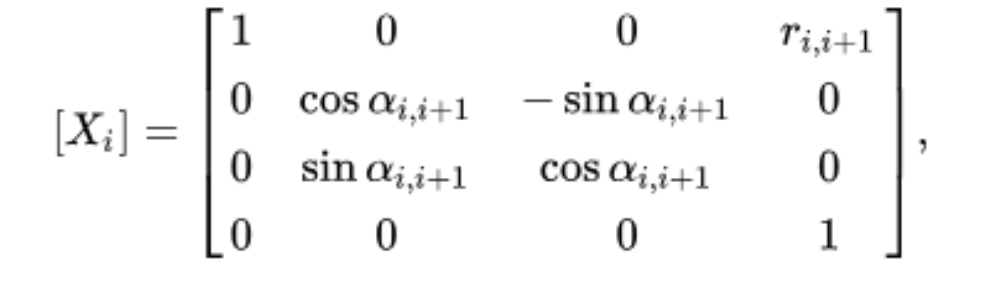
\includegraphics[width=0.7\textwidth]{xframe.PNG}
                \caption{Rotation Matrix for X axis}
                \label{fig:RotationMatrixXAxis}
            \end{figure}
            where $\alpha$i, i+1 and ri,i+1 define the physical dimensions of the link in terms of the angle measured around and distance measured along the X axis. 
            
            As a rule of thumb, the reference frames should follow the 3 rules below.
            \begin{enumerate}
                \item The Z axis is in the direction of the joint axis
                \item The X axis is parallel to the common normal. If there is no unique common normal or the axes are parallel then d becomes a free parameter.
                \item The Y axis completes the reference frame in accordance to the right-handed coordinate frame system.
            \end{enumerate}
            
            A screw displacement can be separated into the product of its translation and rotation about a line. This also helps better explain how this convention of forward kinematics is describing the position of each joint. By doing this the Z axis transformations can be described as;
            \begin{equation}
            [Z_i] = Trans_{Z_i}(d_i)Rot_{Z_i}(\theta_i)
            \end{equation}
            And the X axis transformations are;
            \begin{equation}
            [X_i] = Trans_{X_i}(r_{i,i+1})Rot_{X_i}(\alpha_{i,i+1})
            \end{equation}
            Using this notation, each link can be described by a coordinate transformation from the concurrent coordinate system to the previous coordinate system simply by multiplying each of these transformations together resulting in;
            \begin{equation}
            ^{n-1}T_n=Trans_{z_{n-1}}(d_n)*Rot_{z_{n-1}}(\theta_n)*Trans_{x_n}(r_n)*Rot_{x_n}(\alpha_n)
            \end{equation}
            Breaking each of these transformations into there matrix transformations we get;
            \begin{figure}[H]
                \centering
                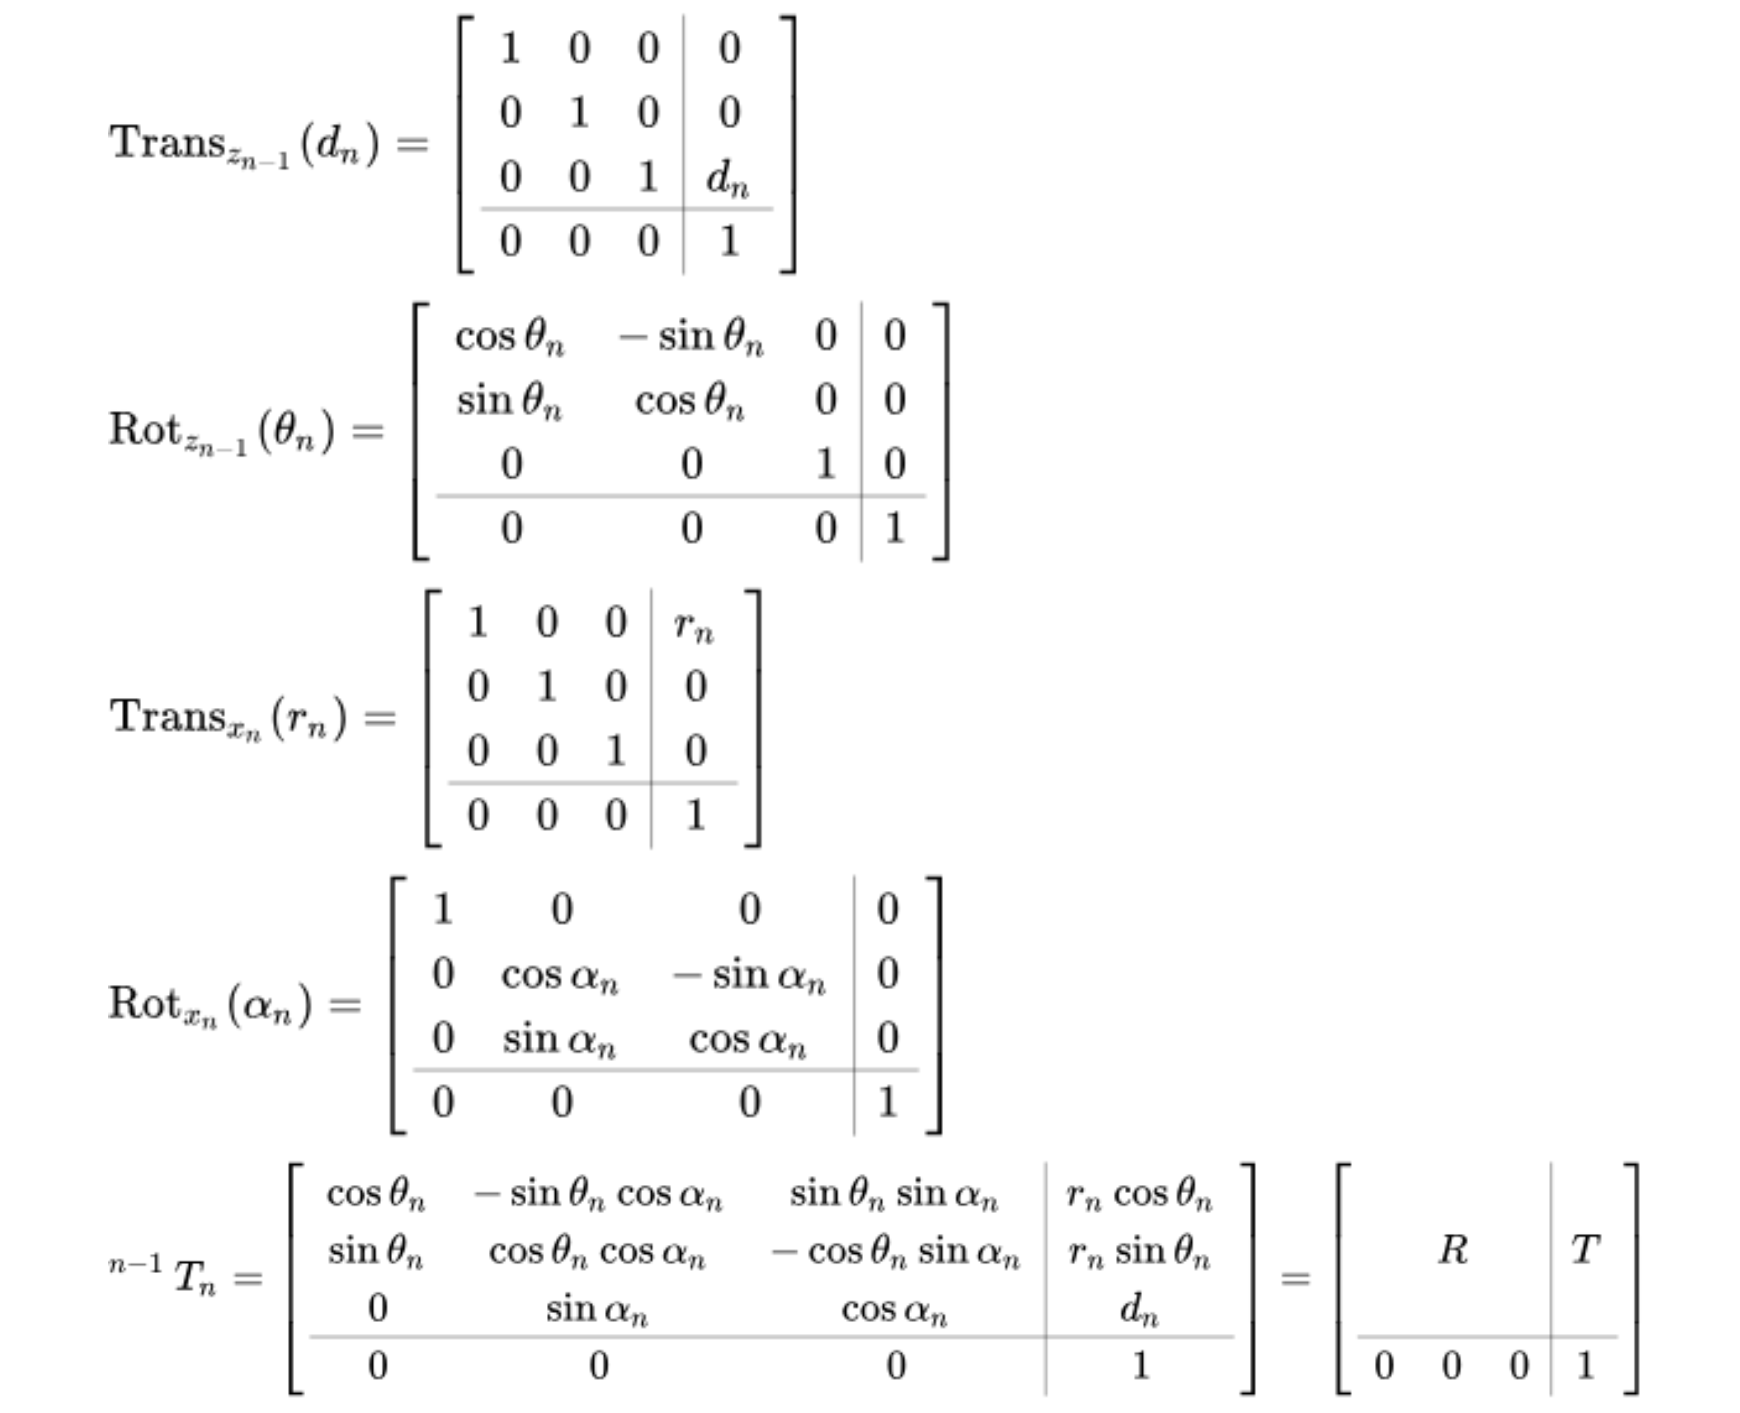
\includegraphics[width=150mm]{Transformation.PNG}
                \caption{Breakdown of transformation matrix}
                \label{fig:TransformationMatrixBreakdown}
            \end{figure}
            At this point we can introduce the actual D-H parameters They were briefly mentioned above when describing the screw displacements but are described below;
            \begin{itemize}
                \item d: offset along previous  z to the common normal
                \item $\theta$: angle about previous z, from old x to new x
                \item r or a: length of the common normal a.. Assuming a revolute joint, this is the radius about previous z.
                \item $\alpha$ angle about common normal, from old z axis to new z axis
            \end{itemize}
            Combining everything we have discussed, the screw displacement, transformation matrix and d-h parameters we get a matrix that looks like the following;
            \begin{figure}[H]
                \centering
                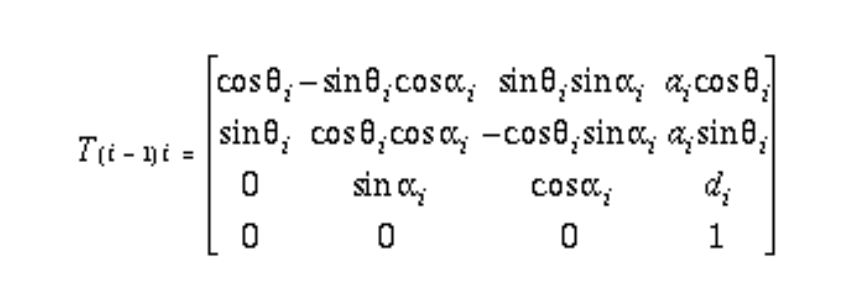
\includegraphics[width=0.7\textwidth]{Matrizx.PNG}
                \caption{Transformation matrix}
                \label{fig:TransformationMatrix}
            \end{figure}
            By placing reference frames using the rules above and using this matrix, the forward kinematics of any serial manipulator can be easily determined where the x,y,z of the end effector is described as the 3x1 matrix $[T_x; T_y; T_z]$ in the result of the final matrix; 
            \begin{figure}[H]
                \centering
                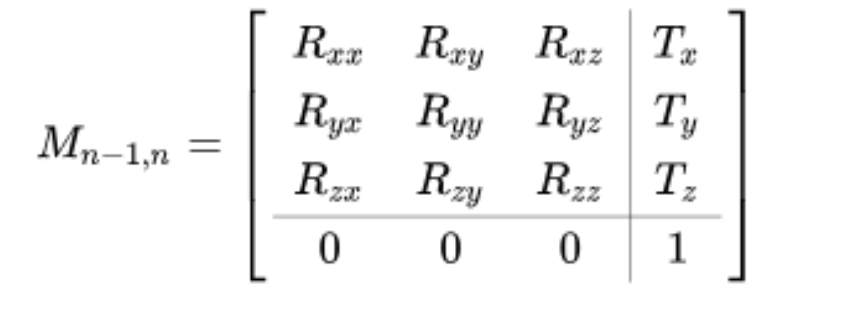
\includegraphics[width=0.7\textwidth]{Matrix2.PNG}
                \caption{Resulting matrix}
                \label{fig:ResultingMatrix}
            \end{figure}
        \subsubsection{Kinematics}
        Kinematics is  often referred to as the geometry of motion and describes the motion of points, bodies and systems of bodies without considering the forces that describe the motion. A kinematics problem begins by describing the geometry of the system and declaring the initial conditions of any known values of position, velocity and/or acceleration of points within the system. Then, using arguments from geometry, the position, velocity and acceleration of any unknown parts of the system can be determined. Using kinematics there are a variety of different calculations that can be done to help create an accurate and useful model of a robot. 
            \paragraph*{Forward Kinematics}
            Forward Kinematics refers to the use of kinematic equations to determine the position, usually in x, y, z coordinate space, of an end effector given specific joint parameters with relation to a specific reference point. In the case of a serial manipulator, this is very useful in understanding where the end of the robot will be if given a set of joint values. There are many different ways of calculating forward kinematics, however one of the most universally accepted and used methods is through the use of Denavit–Hartenberg parameters (DH parameters).
            \begin{figure}[H]
                \centering
                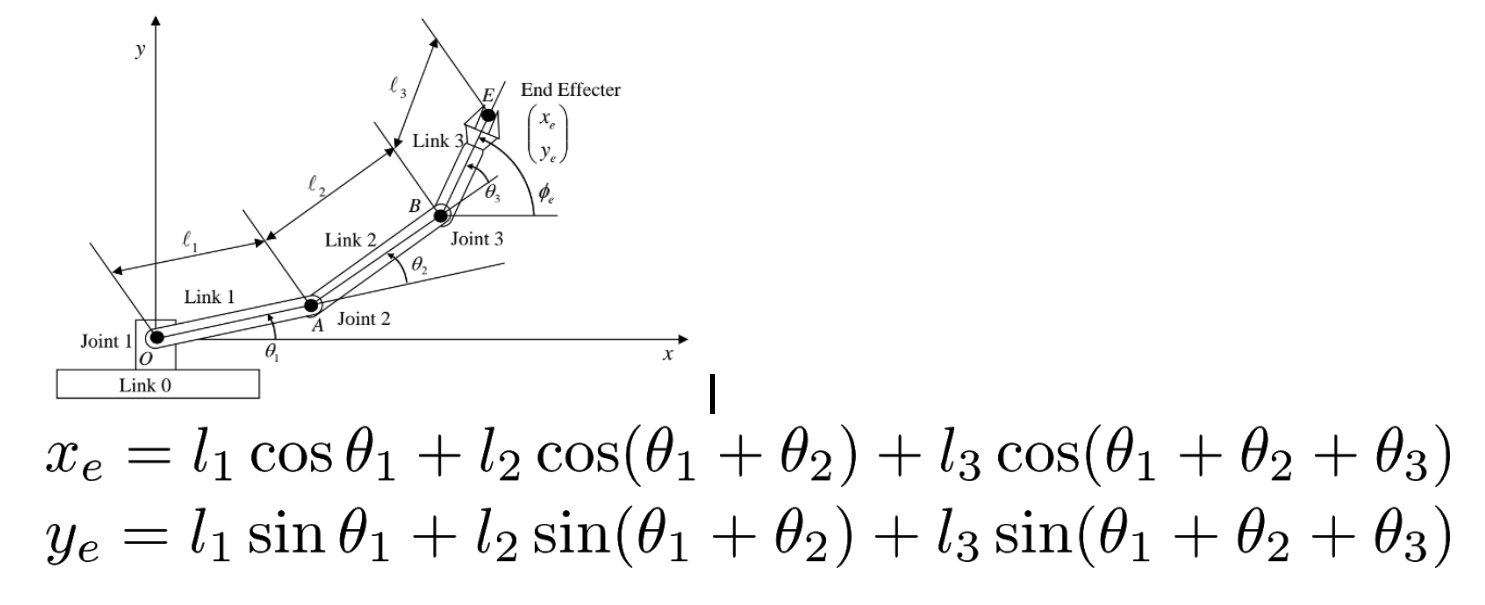
\includegraphics[width=0.8\textwidth]{3dof.PNG}
                \caption{Forward Kinematic equations for a 3 DOF system}
                \label{fig:FWKIN_3DOF}
            \end{figure}
            \paragraph*{Inverse Kinematics}

        \subsubsection{Jacobians}

        \subsubsection{Torque Propogation}

        \subsubsection{Dynamics}
            \paragraph*{The Jacobian}

            \paragraph*{Gravity Compensation \& Coriolis Constants}

        \subsubsection{Basics of Gaits}
            \paragraph*{What is a gait}
            Gait is the pattern of movement of the limbs of animals. Most animals use a variety of gaits, selecting gait based on speed, terrain, the need to maneuver, and energetic efficiency. \cite{wikipedia_2018_Gaits} 

            \paragraph*{Types of gaits}
            There are two general categories of gaits under which all others fall, these are Symmetric and Asymmetric gaits. A symmetric gait is defined when the left and right limbs alternate. where as an asymmetric gait, the legs move in unison. Examples of these gaits can be seen below.  
            \begin{figure}[H]
                \centering
                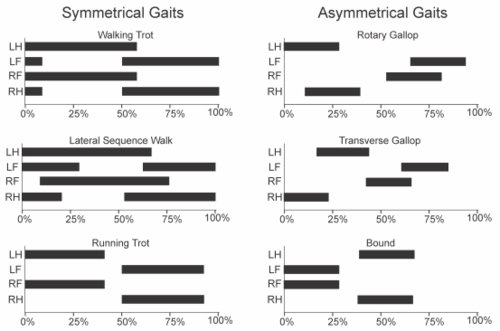
\includegraphics[width=0.7\textwidth]{figures/Gait_graphs_v2.png}
                \caption{Graphic showing motion in types of gaits}
                \label{fig:GaitMotion}
            \end{figure}

        \subsubsection{Dynamic Walking}
            % Fill with research from the grad paper
            % Talk about CPG & paper from grad class

    \subsection{Boston Dynamics Meeting} %% I don't like this name... we should think of another one
        During the course of the project we reached out to Boston Dynamics and arranges a conference call between our team and a group of their engineers from the spot team. We chose to reach out tho them as they are the current leader in the quadrupedal robotics field and would therefore have the most insight into the intricacies and problems that arise in the development of such a platform. We entered the meeting with a series of questions and subordinate related questions. This list comprised of:
        \begin{itemize}
            \item Why was the decision mate to pursue 3DOF legs instead of 4DOF as most quadrupedal animals have. 
            \begin{itemize}
                \item Why did you choose to abstain from a head and tail for balance and dynamics
                \item What are some of the different gaits you have developed and why did you choose them
                \item How have you obtained such a smooth waling gait.
            \end{itemize}
            \item How are your trajectories and kinematics calculated pragmatically
                \begin{itemize}
                    \item Is a real time physics engine used
                    \item Are jacobians calculated at run time
                \end{itemize}
            \item What kind of sensors are used on Spot mini
                \begin{itemize}
                    \item How is each sensor integrated and used for corrections
                    \item recommendations on where to locate each kind of sensor
                \end{itemize}
            \item How importance is torque control in dynamic gaits
            \item What was the minimum control loop speed you found was necessary for smooth operation
        \end{itemize}
        These questions stemmed a very informative conversation between ourselves and the team of engineers which comprised of 2 Electrical engineers and 1 Mechanical engineer, sadly no controls engineers were able to participate however those in attendance were very knowledgeable and were able to answer the majority of our controls related questions. From this conversation we gained a great deal of insight into the tough process that went into developing Spot mini as well as many previous robots in the Spot and big dog series. 

        We started off by asking about the decisions that led to them choosing to only use 3 DOF legs instead of using 4 DOF legs as most quadrupedal animals in nature do. To this we were promptly responded when possible keep the mechanism and calculations as simple as possible, they had tested 4DOF legs on previous robots and found they generally avoided using them and that everything they needed to do could be achieved using 3 DOF, In addition using only 3 DOF also cut down on the wiring, and weight in the legs and therefore lowered the inertial mass of the robot making it over all easier to control. They continued on to speak to the benefits of adding a joint near the center of the body in order to act as a spine which would be much more useful when it cam to highly dynamic gaits and motions allowing for the body to fold more and allow for a smoother transference of momentum.

        This followed into the choice of force sensing, For the project we chose to use an array of barometric pressure sensors encapsulated in polyurethane to calculate a pressure vector. The engineers at Boston dynamics had actually tested a similar kind of sensor and had a great deal of issues using them of their robots as the repetitive motion in walking would either damage of change the calibration of the sensor. In combination with this the temperature of the environment had a great effect of the polyurethanes ability to transmit the applied force to the sensors. This combined with the damage that would get caused to the polyurethane during outdoor testing led them to decide not to continue using this method of sensing. Instead they choose to sense force at the actuator. Their recommendation was to use current to propagate torque at the motor as they used a combination of this and a custom force sensor that they could not speak too much to due to it being part of their "robot secret sauce". 

        Following this we asked about the development of gaits and their choice of a trot gait in which the legs are moves in a FR, BL, BR, FL sequence instead of a more natural pace gait in which the legs are moved in a FR, BR, FL, BL sequence. Their response was different to what we had expected, in end Spot is able to perform a pace gait however it is less stable than the trot gait. The trot gait was the first successful gait the team was able to develop when working on the original spot project and therefore has had the most development put into it. Further gait development came with difficulties, the development of a bounding or galloping gait was severely hindered by the lack of an effective spine, without this the body would form an oscillating system making the robot unstable. However when mentioned the concept of a continuum spine which would result in the greatest mobility they greatly recommended against it, this was due to the uncertainty and inability to guarantee the position of the system for a given input. For all dynamic motions such as recovering from a push or jerk, they rely heavily on the IMU which in a ridged body robot they recommend placing it directly over the center of the robot however for a split body or one using a spine they recommended placing one on each segment in order to capture the motion of each independent system. 
        
        Leading from this to kinematics and trajectory planning allowed us to learn that they do use both a simulation and a real time physics engine as well as calculation all necessary jacobians at run time. This led us to asking details of their control feedback and they recommended getting a high level controller running at \~1 kHz for a smooth trajectory and a low level controller as fast as possible in order to have a stable PID loop and remove all gittering and jerkiness from the system. 
    
%%%%% this is the end